\documentclass{article}

% Needs to be loaded before cleveref, so we can specify the name
% of a `listing` environment (https://tex.stackexchange.com/a/47694)
\usepackage{listings}
%%% Local Variables:
%%% mode: latex
%%% TeX-master: "../main"
%%% End:

% Recommended, but optional, packages for figures and better typesetting:
\usepackage{microtype}
\usepackage{graphicx}
\usepackage{booktabs} % for professional tables

% hyperref makes hyperlinks in the resulting PDF.
% If your build breaks (sometimes temporarily if a hyperlink spans a page)
% please comment out the following usepackage line and replace
% \usepackage{icml2024} with \usepackage[nohyperref]{icml2024} above.
\usepackage{hyperref} % hyperlinks

% Attempt to make hyperref and algorithmic work together better:
\newcommand{\theHalgorithm}{\arabic{algorithm}}

% Use the following line for the initial blind version submitted for review:
% \usepackage{icml2024}

% If accepted, instead use the following line for the camera-ready submission:
\usepackage[accepted]{icml2024}

% For theorems and such
\usepackage{amsmath}
\usepackage{amssymb}
\usepackage{mathtools}
\usepackage{amsthm}

% if you use cleveref..
\usepackage[capitalize,noabbrev]{cleveref}

%%%%%%%%%%%%%%%%%%%%%%%%%%%%%%%%
% THEOREMS
%%%%%%%%%%%%%%%%%%%%%%%%%%%%%%%%
\theoremstyle{plain}
\newtheorem{theorem}{Theorem}[section]
\newtheorem{proposition}[theorem]{Proposition}
\newtheorem{lemma}[theorem]{Lemma}
\newtheorem{corollary}[theorem]{Corollary}
\theoremstyle{definition}
\newtheorem{definition}[theorem]{Definition}
\newtheorem{assumption}[theorem]{Assumption}
\newtheorem{example}[theorem]{Example}
\theoremstyle{remark}
\newtheorem{remark}[theorem]{Remark}
%%% Local Variables:
%%% mode: latex
%%% TeX-master: "../main"
%%% End:

\input{preamble/goodfellow.tex}
% ===================================================================
% WRITING
% ===================================================================
\usepackage{paracol}
\usepackage{blindtext}
\newcommand{\felix}[1]{\textcolor{red}{Felix: #1}}
\newcommand{\balint}[1]{\textcolor{orange}{Bálint: #1}}

% ===================================================================
% COLORS
% ===================================================================
% VECTOR PRIMARY COLORS
\definecolor{VectorBlack}{RGB}{34, 34, 34}
\definecolor{VectorGray}{RGB}{239, 238, 237}

% VECTOR SECONDARY COLORS
\definecolor{VectorBlue}{RGB}{59, 69, 227}
\definecolor{VectorPink}{RGB}{253, 8, 238}
\definecolor{VectorOrange}{RGB}{250, 173, 26}
\definecolor{VectorTeal}{RGB}{82, 199, 222}

% ===================================================================
% REFERENCES
% ===================================================================
\hypersetup{%
  colorlinks,
  citecolor = VectorBlue,%
  linkcolor = VectorBlue,%
  urlcolor = VectorPink,%
}%
% tell cleveref how to name a listing environment
\crefname{listing}{snippet}{snippets}
% Rename Listing into Snippet
\renewcommand{\lstlistingname}{Snippet}

% ===================================================================
% CODE BLOCKS
% ===================================================================
% define style for listings using the Vector color scheme
\lstdefinestyle{vector_institute}{
  backgroundcolor=\color{VectorGray!50},
  commentstyle=\bfseries\color{VectorBlue},
  keywordstyle=\bfseries\color{VectorBlack},
  numberstyle=\tiny\color{VectorBlack!50},
  stringstyle=\bfseries\color{VectorPink},
  basicstyle=\ttfamily\scriptsize,
  xleftmargin=3.2ex,
  breakatwhitespace=false,
  breaklines=true,
  captionpos=t,
  keepspaces=true,
  numbers=left,
  numbersep=7pt,
  showspaces=false,
  showstringspaces=false,
  showtabs=false,
  tabsize=2,
  escapebegin={\color{blue}},
  linewidth=\linewidth,
  mathescape=true,
}
% use the above style as default
\lstset{style=vector_institute}

\usepackage{caption}
% modify captions of code blocks
\captionsetup[lstlisting]{%
  font={scriptsize},%
  justification=raggedright,%
  singlelinecheck=false,%
}

% \usepackage{minted}
% \usemintedstyle{emacs}

\newcommand{\repourl}{https://github.com/f-dangel/kfac-from-scratch}
% Command to include code blocks and their output.
% First argument is the filename inside the kfac_tutorial directory.
% The listing can be referenced with that filename, too.
\newcommand{\codeblock}[1]{
  % convert _ into \_ for LaTeX
  \def\filename{\detokenize{#1}}
  % \inputminted[%
  % fontsize=\scriptsize,%
  % % obeytabs,%
  % tabsize=0,%
  % bgcolor=VectorGray!50,%
  % texcomments=true,%
  % ]{python}{../kfs/#1.py}
  \lstinputlisting[%
  language=python,%
  caption=\href{\repourl/kfs/#1.py}{\texttt{kfs/\filename.py}},%
  label=#1,%
  ]{../kfs/#1.py}
  % \vspace{-1.25\baselineskip}
  % \lstinputlisting[%
  % language=python,%
  % numbers=none,%
  % basicstyle=\bfseries\ttfamily\scriptsize,%
  % title=\href{\repourl/tex/output/#1.txt}{Output:}\hfill,%
  % ]{output/#1.txt}
}

% ===================================================================
% MATH
% ===================================================================
\usepackage{nicefrac}
\DeclareMathOperator{\rvec}{rvec}
\DeclareMathOperator{\cvec}{cvec}
\let\vec\relax % delete the existing \vec command
\DeclareMathOperator{\vec}{vec}
\DeclareMathOperator{\mat}{mat}
\DeclareMathOperator{\lin}{lin}

\usepackage{mdframed}
\mdfdefinestyle{custom}{%
  linecolor=black,%
  topline=false,%
  bottomline=false,%
  rightline=false,%
  linewidth=1.25pt,%
  backgroundcolor=VectorGray!50,%
  innerleftmargin=5pt,%
  % innertopmargin=8pt,%
}
\theoremstyle{definition}
\newmdtheoremenv[style=custom]{definition}{Definition}[section]
\newmdtheoremenv[style=custom]{setup}{Setup}[section]
\newmdtheoremenv[%
style=custom,%
linecolor=VectorOrange,%
backgroundcolor=VectorOrange!10,%
]{caveat}{Caveat}[section]
\newmdtheoremenv[%
style=custom,%
linecolor=VectorTeal,%
backgroundcolor=VectorTeal!10,%
]{test}{Test}[section]
\newmdtheoremenv[%
style=custom,%
linecolor=VectorTeal,%
backgroundcolor=VectorTeal!10,%
]{example}{Example}[section]

% ===================================================================
% FIGURES
% ===================================================================
\usepackage{tikz}
\usetikzlibrary{arrows.meta}
\usetikzlibrary{positioning}

%%% Local Variables:
%%% mode: latex
%%% TeX-master: "../main"
%%% End:


\begin{document}

% By default, paracol defines all counters to be local per column.
% The following makes it use a single global counter for figures.
% See https://tex.stackexchange.com/a/304466 for details.
\globalcounter{figure}
\globalcounter{example}

\onecolumn
\newcommand{\papertitle}{%
  Kronecker-factored Approximate Curvature (KFAC) From Scratch
}%
\title{\papertitle}

% The \icmltitle you define below is probably too long as a header.
% Therefore, a short form for the running title is supplied here:
\icmltitlerunning{\papertitle}

\icmltitle{\papertitle}

% It is OKAY to include author information, even for blind
% submissions: the style file will automatically remove it for you
% unless you've provided the [accepted] option to the icml2024
% package.

% List of affiliations: The first argument should be a (short)
% identifier you will use later to specify author affiliations
% Academic affiliations should list Department, University, City, Region, Country
% Industry affiliations should list Company, City, Region, Country

% You can specify symbols, otherwise they are numbered in order.
% Ideally, you should not use this facility. Affiliations will be numbered
% in order of appearance and this is the preferred way.
\icmlsetsymbol{equal}{*}

\begin{icmlauthorlist}
\icmlauthor{Felix Dangel}{equal,vector}
\icmlauthor{Runa Eschenhagen}{equal,cambridge}
\icmlauthor{B\'alint Mucs\'anyi}{equal,tue}
\icmlauthor{Tobias Weber}{equal,tue}
\end{icmlauthorlist}

\icmlaffiliation{vector}{Vector Institute, Canada}
\icmlaffiliation{cambridge}{University of Cambridge, United Kingdom}
\icmlaffiliation{tue}{University of T\"ubingen, Germany}

\icmlcorrespondingauthor{Felix Dangel}{fdangel@vectorinstitute.ai}
% \icmlcorrespondingauthor{Firstname2 Lastname2}{first2.last2@www.uk}

% You may provide any keywords that you
% find helpful for describing your paper; these are used to populate
% the "keywords" metadata in the PDF but will not be shown in the document
\icmlkeywords{KFAC, Natural gradient descent}

\vskip 0.3in

% this must go after the closing bracket ] following \twocolumn[ ...

% This command actually creates the footnote in the first column
% listing the affiliations and the copyright notice.
% The command takes one argument, which is text to display at the start of the footnote.
% The \icmlEqualContribution command is standard text for equal contribution.
% Remove it (just {}) if you do not need this facility.

% \printAffiliationsAndNotice{}  % leave blank if no need to mention equal contribution
\printAffiliationsAndNotice{\icmlEqualContribution} % otherwise use the standard text.
%%% Local Variables:
%%% mode: latex
%%% TeX-master: "../main"
%%% End:
 % Creates title

\vspace*{-2ex}

% logo
\begin{center}
\begin{tikzpicture}
    \node[inner sep=0.7pt, opacity=0.5, draw opacity=1, draw=black!50!white, ultra thick, rounded corners]{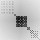
\includegraphics[scale=0.66]{figures/logo.pdf}};
\end{tikzpicture}
\end{center}

\vfill

\begin{abstract}
  Kronecker-factored approximate curvature \citep[KFAC,][]{martens2015optimizing} is arguably one of the most prominent curvature approximations in deep learning.
  Its applications range from optimization to Bayesian deep learning, training data attribution with influence functions, and model compression or merging.
  While the intuition behind KFAC is easy to understand, its implementation is tedious: It comes in many flavours, has common pitfalls when translating the math to code, and is challenging to test, which complicates ensuring a properly functioning implementation.
  Some of the authors themselves have dealt with these challenges and experienced the discomfort of not being able to fully test their code.
  Thanks to recent advances in understanding KFAC, we are now able to provide test cases and a recipe for a reliable KFAC implementation.
  \emph{This tutorial is meant as a ground-up introduction to KFAC.}
  In contrast to the existing work, our focus lies on providing both math and code side-by-side and providing test cases based on the latest insights into KFAC that are scattered throughout the literature.
  We hope this tutorial provides a contemporary view of KFAC that
  allows beginners to gain a deeper understanding of this curvature approximation while lowering the barrier to its implementation, extension, and usage in practice.
\end{abstract}

\vfill

\paragraph{Version:} \today\,(v1.0.0)

\paragraph{About the length of this document.}
Before you close this document because you saw the page count:
the \emph{effective length is much shorter than suggested by its page number}.
This is because \emph{we use an experimental two-column layout which presents text and code in parallel} and leads to a large amount of white space.
The left column contains the main text with explanations and mathematical descriptions.
The right column accompanies the left one with code snippets to make the ideas precise in code; it can safely be skipped if you are in a rush.
And if you already know the basics, it suffices to read the KFAC-specific part (Pages \pageref{sec:kfac-overview}--\pageref{sec:kfac-cheatsheet}).

\paragraph{Follow along in code.} The \LaTeX\,\& Python source code is available at~\href{\repourl}{\texttt{github.com/f-dangel/kfac-tutorial}}.
This allows you to run the code as you read:
Clone the repository and follow the installation instructions.
You can then run each snippet from the repository root, for instance by calling \texttt{python kfs/basics/forward\_pass.py}.
If you find typos or have suggestions for improving explanations, math, or code, please open issues and pull requests.
In doing so, you are contributing to making this tutorial a valuable reference for newcomers.

\vspace{\baselineskip}
%%% Local Variables:
%%% mode: latex
%%% TeX-master: "../main"
%%% End:

\clearpage

\section*{How to read this document?}

\paragraph{Layout} This document has a somewhat unusual structure in that it uses a parallel column format.
The left column contains the main text with explanations and mathematical descriptions.
The right column accompanies the left one with code snippets to make the ideas precise in code.
It can safely be skipped if you are in a rush.

\begin{figure*}[!h]
  \centering
  \section*{How to read this document?}

\paragraph{Layout} This document has a somewhat unusual structure in that it uses a parallel column format.
The left column contains the main text with explanations and mathematical descriptions.
The right column accompanies the left one with code snippets to make the ideas precise in code.
It can safely be skipped if you are in a rush.

\begin{figure*}[!h]
  \centering
  \section*{How to read this document?}

\paragraph{Layout} This document has a somewhat unusual structure in that it uses a parallel column format.
The left column contains the main text with explanations and mathematical descriptions.
The right column accompanies the left one with code snippets to make the ideas precise in code.
It can safely be skipped if you are in a rush.

\begin{figure*}[!h]
  \centering
  \input{figures/reading_guide.tex}
\end{figure*}
%%% Local Variables:
%%% mode: LaTeX
%%% TeX-master: "../main"
%%% End:

\end{figure*}
%%% Local Variables:
%%% mode: LaTeX
%%% TeX-master: "../main"
%%% End:

\end{figure*}
%%% Local Variables:
%%% mode: LaTeX
%%% TeX-master: "../main"
%%% End:

\clearpage

% Show sections and subsections in TOC
\setcounter{tocdepth}{2}
\tableofcontents
\clearpage

\section{Preface}\label{sec:preface}
This is an attempt to bundle scattered knowledge about KFAC into a single document, explain all the technicalities and pitfalls, and present tests to ensure bug-free implementations.

Should answer the following questions:
\begin{itemize}
\item Why do we need this tutorial?
\item Why is this not a Jupyter notebook?
\item What do we gain by explaining KFAC bottom-up?
\item What ML framework do we use and why?
\item What are we \emph{not} doing (e.g.\,building an optimizer)?
\end{itemize}

We use PyTorch~\cite{paszke2019pytorch} and implement everything using \texttt{torch.nn} rather than a functional formulation as we feel that many deep learning practitioners are more familiar with this style.
There could be a JAX or functorch version, too.

\begin{itemize}
\item KFAC approximates the Fisher, which is an outer product of gradients. The gradients involve the output-parameter Jacobian of a weight, which has Kronecker structure,
  \begin{align}
    \jac_{\mW}(\mW \vx) = \vx^{\top} \otimes \mI\,.
  \end{align}
  This implies that the Fisher contains terms of the following form, where $\bullet$ is a placeholder for some matrix,
  \begin{align}
    \left(
    \vx^{\top}\otimes \mI
    \right)^{\top}
    \bullet
    \left(
    \vx^{\top}\otimes \mI
    \right)\,.
  \end{align}

\item The goal is to build up to an abstract general formulation of KFAC.
  Given a compute graph which uses the operations $\vx, \mW \mapsto \mW x$, potentially in multiple places, define a Kronecker approximation of the Fisher.
  Also to show the different degrees of freedom: treating weights \& biases jointly/separately, using reduce versus expand approximation, and treating weight tying, i.e.
  multi-usage of $\mW$.

\end{itemize}
TODO Should mention somewhere that many of the provided examples are already discussed in Felix's PhD thesis~\cite{dangel2023backpropagation}.

\paragraph{KFAC flavours} There are various degrees of freedom that induce different KFAC flavours:
\begin{align*}
  \begin{array}{c}
    \begin{Bmatrix}
      \text{PyTorch}
      \\
      \text{JAX}
    \end{Bmatrix}
    \\
    \text{(software framework)}
  \end{array}
  \times
  \begin{array}{c}
    \begin{Bmatrix}
      \rvec
      \\
      \cvec
    \end{Bmatrix}
    \\
    \text{(flattening convention)}
  \end{array}
  \times
  \begin{array}{c}
    \begin{Bmatrix}
      \text{MC (type-I Fisher)}
      \\
      \text{type-II Fisher}
      \\
      \text{empirical Fisher}
    \end{Bmatrix}
    \\
    \text{(target curvature)}
  \end{array}
  \times
  \begin{array}{c}
    \begin{Bmatrix}
      \text{expand}
      \\
      \text{reduce}
    \end{Bmatrix}
    \\
    \text{(how weight sharing is handled)}
  \end{array}
  \times
  \begin{array}{c}
    \begin{Bmatrix}
      \text{fully-connected}
      \\
      \text{convolutions}
    \end{Bmatrix}
    \\
    \text{(layers)}
  \end{array}
\end{align*}
The original work from~\citet{martens2015optimizing} uses
\begin{align*}
  \text{cvec} \times \text{MC (type-I Fisher)} \times \text{expand} \times \text{fully-connected}\,.
\end{align*}
\paragraph{Version 1.0} This document aims to provide an introduction to the following flavours:
\begin{align*}
  \text{PyTorch}
  \times
  \begin{Bmatrix}
    \rvec
    \\
    \cvec
  \end{Bmatrix}
  \times
  \begin{Bmatrix}
    \text{MC (type-I Fisher)}
    \\
    \text{type-II Fisher}
    \\
    \text{empirical Fisher}
  \end{Bmatrix}
  \times
  \text{expand}
  \times
  \text{fully-connected}
\end{align*}
This allows us to (i) highlight challenges when translating math to code, (ii) pointing out various connections between the curvature matrices and KFAC, and (iii) produce a working, tested, version of the original KFAC paper with slight generalizations.
%%% Local Variables:
%%% mode: latex
%%% TeX-master: "../main"
%%% End:

\clearpage

\columnratio{0.42}
\begin{paracol}{2}
  \section{Basics}\label{sec:basics}
  \subsection{Empirical risk minimization \& Maximum Likelihood Estimation}

\begin{paracol}{2}

  \begin{align}
    \gL(\vtheta) &= \sum_{n=1}^N \ell(\vtheta, \vx_n, \vy_n)
    \\
                 &=
                   \sum_{n=1}^N c(f(\vtheta, \vx_n), \vy_n)
  \end{align}

  \switchcolumn[0]

  \blindtext

  \switchcolumn[1]

  \switchcolumn[0]* % sync

  \blindtext

  \switchcolumn[1]

  \codeblockWithOutput{hello_world}

  \switchcolumn[0]

  \Cref{hello_world} says hello world.

  \subsection{Derivatives}

  \begin{caveat}
    In deep learning, we often work with matrices, or higher-dimensional tensors.
    We want to use matrix linear algebra expressions to avoid using heavy index notation.
    This can be achieved by flattening all tensors back into vectors and re-using definitions derivatives from the vector case.
    However, we must be careful when translating the results back to the tensor format, as the translation process depends on the flattening convention.
    Classically, the mathematical derivations prefer a \emph{different} flattening scheme than the one used in deep learning libraries.
  \end{caveat}

  \switchcolumn[0]*
  \subsubsection{Flattening}

  There are two popular flattening conventions: last-varies-fastest and first-varies-fastest.

  \begin{example}
    For matrix
    \(
    \mA = \begin{pmatrix}
            1 & 2 \\
            3 & 4
          \end{pmatrix}
          \), we have
          \begin{equation*}
            \rvec(\mA)
            =
            \begin{pmatrix}
              1 \\ 2 \\ 3 \\ 4
            \end{pmatrix}\,,
            \qquad
            \cvec(\mA)
            =
            \begin{pmatrix}
              1 \\ 3 \\ 2 \\ 4
            \end{pmatrix}\,,
          \end{equation*}
          see \Cref{flattening}.
        \end{example}

        \switchcolumn[1]
        \codeblockWithOutput{flattening}

        \switchcolumn[0]*
        \subsubsection{Jacobians, JVP, VJPs}

        \begin{definition}[Jacobian]
          Consider a vector-to-vector function $f: \sR^A \to \sR^B, \va \mapsto \vb = f(\va)$.
          Its Jacobian $\jac_{\va}\vb \in \sR^{\mB \times \mA}$ collects the first-order partial derivatives into a matrix such that
          \begin{align*}
            [\jac_{\va} \vb]_{i,j} = \frac{\partial [f(\va)]_i}{\partial [\va]_j}\,.
          \end{align*}
        \end{definition}

        \begin{definition}[General Jacobian]
          TODO
        \end{definition}

        \begin{definition}[Vector-Jacobian products]
          TODO
        \end{definition}

        \begin{definition}[$\cvec$-Jacobian]
          Consider a tensor-to-tensor function $f: \sR^{A_1 \times \dots \times A_N} \to \sR^{B_1 \times \dots \times B_M}, \tA \mapsto \tB = f(\tA)$. Its $\cvec$-Jacobian $\jac^{\cvec}_{\tA}\tB \in \sR^{A_N \cdots A_1 \times B_M \cdots B_1}$ results from flattening input and output tensors with $\cvec$ and applying the Jacobian definition for vectors,
          \begin{align*}
            [\jac^{\cvec}_{\tA}\tB]_{i,j}
            =
            \frac{\partial [\cvec(f(\tA))]_i}{\partial [\cvec(\tA)]_j}\,.
          \end{align*}
        \end{definition}

        \begin{definition}[$\rvec$-Jacobian]
          Consider a tensor-to-tensor function $f: \sR^{A_1 \times \dots \times A_N} \to \sR^{B_1 \times \dots \times B_M}, \tA \mapsto \tB = f(\tA)$. Its $\cvec$-Jacobian $\jac^{\cvec}_{\tA}\tB \in \sR^{A_1 \cdots A_N \times B_1 \cdots B_M}$ results from flattening input and output tensors with $\cvec$ and applying the Jacobian definition for vectors,
          \begin{align*}
            [\jac^{\cvec}_{\tA}\tB]_{i,j}
            =
            \frac{\partial [\cvec(f(\tA))]_i}{\partial [\cvec(\tA)]_j}\,.
          \end{align*}
        \end{definition}

        \switchcolumn[1]
        \codeblockWithOutput{jacobians}


        \switchcolumn[1]*
        \codeblockWithOutput{jacobians_linear_layer}
        \switchcolumn[0]

        \begin{example}[$\cvec$- and $\rvec$-weight Jacobians of a linear layer]
          Consider an affine map with weight matrix $\mW \in \sR^{D_{\text{out}} \times D_{\text{in}}}$, bias vector $\vb \in \sR^{D_{\text{out}}}$, input vector $\vx \in \sR^{D_{\text{in}}}$ and output vector $\vz \in \sR^{D_{\text{out}}}$ with
          \begin{align*}
            \vz
            \coloneqq
            \mW \vx + \vb
            =
            \begin{pmatrix}
              \mW & \vb
            \end{pmatrix}
            \begin{pmatrix}
              \vx \\ 1
            \end{pmatrix}
            \coloneqq
            \tilde{\mW}
            \tilde{\vx}\,.
          \end{align*}
          To express this operation as matrix-vector multiplication, we combined weight and bias into a single matrix $\tilde{\mW}$ and augment the input with a one, yielding $\tilde{\vx}$, to account for the bias contribution.

          The $\cvec$-Jacobian w.r.t.\,the combined weight is
          \begin{align*}
            \jac^{\cvec}_{\tilde{\mW}}\vz
            =
            \tilde{\vx}^{\top}
            \otimes
            \mI_{D_{\text{out}}}\,.
          \end{align*}
          In contrast, the $\rvec$-Jacobian is
          \begin{align*}
            \jac^{\cvec}_{\tilde{\mW}}\vz
            =
            \mI_{D_{\text{out}}}
            \otimes
            \tilde{\vx}^{top}\,,
          \end{align*}
          see \Cref{jacobians_linear_layer}.
          Note that the order of Kronecker factors is \emph{reversed}, depending on the flattening scheme.
        \end{example}

        \begin{example}[$\cvec$- and $\rvec$-weight Jacobians of a linear layer with weight sharing]
          Consider the same affine map from above, but now processing multiple input vectors $\mX = \begin{pmatrix}\vx_1 & \dots & \vx_S\end{pmatrix} \in \sR^{D_{\text{in}}\times S}$, yielding a sequence $\mZ = \begin{pmatrix} \vz_1 & \dots & \vz_S\end{pmatrix} \in \sR^{D_{\text{out}}\times S}$ where each $\vz_s$ is produced like above.
          The parameters are \emph{shared} over all vectors in the input sequence.
          In matrix notation,
          \begin{align*}
            \mZ
            \coloneqq
            \mW \mX + \vb \vone^{\top}_S
            =
            \begin{pmatrix}
              \mW & \vb
            \end{pmatrix}
            \begin{pmatrix}
              \mX \\ \vone^{\top}_S
            \end{pmatrix}
            \coloneqq
            \tilde{\mW}
            \tilde{\mX}\,.
          \end{align*}
          The $\cvec$-Jacobian w.r.t.\,the combined weight is
          \begin{align*}
            \jac^{\cvec}_{\tilde{\mW}}\mZ
            =
            \tilde{\mX}
            \otimes
            \mI_{D_{\text{out}}}\,.
          \end{align*}
          In contrast, the $\rvec$-Jacobian is
          \begin{align*}
            \jac^{\cvec}_{\tilde{\mW}}\mZ
            =
            \mI_{D_{\text{out}}}
            \otimes
            \tilde{\mX}\,,
          \end{align*}
          see \Cref{jacobians_shared_linear_layer}.
        \end{example}

        \switchcolumn[1]
        \codeblockWithOutput{jacobians_shared_linear_layer}

      \end{paracol}
      \subsubsection{Hessians, HVPs}

      \subsection{Curvature Matrices}
      \subsubsection{The Generalized Gauss-Newton (GGN)}
      \subsubsection{The Fisher}
      \subsubsection{The Connection between GGN \& Fisher}
      \subsubsection{The Empirical Fisher (EF)}

      %%% Local Variables:
      %%% mode: latex
      %%% TeX-master: "../main"
      %%% End:

  \switchcolumn[0]*
\end{paracol}
\clearpage

\begin{paracol}{1}
  \section{Cheatsheet: Basics}\label{sec:cheatsheet-basics}
  \begin{itemize}
\item Risk minimization and tractable empirical risk minimization (\Cref{subsec:empirical-risk-minimization})
  \begin{align*}
    \argmin_{\vtheta} \gL_{p_{\text{data}}(\rvx, \rvy)}(\vtheta)
    \qquad
    &\text{where}\qquad
      \gL_{p_{\text{data}}(\rvx, \rvy)}(\vtheta) \coloneq \E_{(\vx, \vy) \sim p_{\text{data}}(\rvx, \rvy)}
      \left[
      c(f(\vx, \vtheta), \vy)
      \right]
    &\text{(intractable)}
      \shortintertext{(use empirical density $p_{\sD}(\rvx, \rvy) = \frac{1}{N} \sum_n \delta(\rvx - \vx_n) \delta(\rvy - \vy_n)$ from data $\sD = \{ (\vx_n, \vy_n) \sim p_{\text{data}} \mid n=1, \dots, N \}$)}
      \argmin_{\vtheta} \gL_{\sD}(\vtheta)
      \qquad
    &\text{where}\qquad
      \gL_{\sD}(\vtheta) \coloneq R \sum_{n=1}^N c(f(\vx_n; \vtheta), \vy_n)\,.
    &\text{(tractable)}
  \end{align*}
  (changing the reduction factor $R$ does not change the optimization problem's solution)

\item Common criterion functions and their reduction constants (\Cref{ex:square_loss,ex:cross_entropy_loss})
  \begin{align*}
    &\begin{matrix}
      \text{Square loss}
      \\
      \text{(\texttt{MSELoss})}
    \end{matrix}
      \qquad
    &c(\vf, \vy) = \frac{1}{2} \left\lVert \vf - \vy \right\rVert_2^2\,,
      \qquad
    &R =
      \begin{cases}
        2 & \text{\texttt{reduction="sum"}} \\
        \frac{2}{N \dim(\vy)} & \text{\texttt{reduction="mean"}}
      \end{cases}
    \\
    &\begin{matrix}
      \text{Softmax cross-entropy loss}\\
      \text{(\texttt{CrossEntropyLoss})}
    \end{matrix}
      \qquad
    &c(\vf, y) = - \log( [\softmax(\vf)]_y)\,,
      \qquad
    &R =
      \begin{cases}
        1 & \text{\texttt{reduction="sum"}} \\
        \frac{1}{N \dim(\vf)} & \text{\texttt{reduction="mean"}}
      \end{cases}
  \end{align*}

\item Probabilistic interpretation of a neural net: Parameterize $p(\rvx, \rvy \mid \vtheta) = p_{\text{data}}(\rvx) p(\rvy \mid \rvx, \vtheta) = p_{\text{data}}(\rvx) r(\rvy \mid f(\rvx, \vtheta))$
  \begin{align*}
    \argmin_{\vtheta} \mathrm{KL}( p_{\text{data}}(\rvx, \rvy) \mid\mid p(\rvx, \rvy \mid \vtheta) )
    \quad\Leftrightarrow\quad
    &\argmin_{\vtheta} \E_{p_{\text{data}}(\rvx)} \E_{r(\rvy \mid \rvx, \vtheta)} \left[
      - \log r(\rvy \mid f(\rvx, \vtheta))
      \right]
    &\text{(intractable)}
      \shortintertext{(use empirical density to make tractable)}
      \qquad
    &\argmin_{\vtheta} - R \sum_{n=1}^N \log r(\rvy=\vy_n \mid f(\rvx=\vx_n, \vtheta))
    &\text{(tractable)}
  \end{align*}

\item Common criteria are negative log-likelihoods: $c(\vf, \vy) = - \log r(\rvy=\vy \mid f(\rvx, \vtheta) = \vf)$ (\Cref{ex:square_loss_probabilistic,ex:cross_entropy_loss_probabilistic})
  \begin{align*}
    &\text{Square loss (\texttt{MSELoss})}
      \qquad
    &r(\rvy \mid \vf) = \gN( \rvy \mid \vmu = \vf, \mSigma = \mI)
    \\
    &\text{Softmax cross-entropy loss (\texttt{CrossEntropyLoss})}
      \qquad
    &r(\ry \mid \vf) = \gC( \ry \mid \vsigma = \softmax(\vf))
  \end{align*}

\item Shorthands: Per-datum prediction $\vf_n(\vtheta) = f(\vx_n, \vtheta)$, criterion $c_n(\vf_n) = c(\vf_n, \vy_n)$, and loss $\ell_n(\vtheta) = c_n(\vf_n(\vtheta))  $

\item Net Jacobian $\jac_{\vtheta}\vf \in \sR^{\dim(\gF) \times D}$, $[\jac_{\vtheta} \vf]_{i,j} = \frac{\partial [\vf]_i}{\partial [\vtheta]_j}$, criterion Hessian $\hess_{\vf} c \in \sR^{\dim(\gF) \times \dim(\gF)}$, $[\hess_{\vf}c]_{i,j} = \frac{\partial^2 c}{\partial [\vf]_i \partial [\vf]_j}$

\item Hessian, generalized Gauss-Newton, type-II/I/empirical Fishers ($\vf_n \coloneq f(\vx_n, \vtheta)$, $\rvf = f(\rvx, \vtheta)$, $\tilde{\vy}_{n,m} \sim r(\rvy \mid \rvf = \vf_n)$)
  \begin{align*}
    \hess_{\vtheta} \gL(\vtheta)
    &= R \sum_{n=1}^N \hess_{\vtheta} c(\vf_n, \vy_n)
      = -R \sum_{n=1}^N \hess_{\vtheta} \log r(\rvy = \vy_n \mid \rvf = \vf_n)
    \\
    \mG(\vtheta)
    &= R \sum_{n=1}^N
      \jac_{\vtheta} \vf_n^{\top}
      \left(
      \hess_{\vf_n} c(\vf_n, \vy_n)
      \right)
      \jac_{\vtheta} \vf_n
      =
      R \sum_{n=1}^N
      \jac_{\vtheta} \vf_n^{\top}
      \left(
      -\hess_{\vf_n} \log r(\rvy = \vy_n \mid \rvf = \vf_n)
      \right)
      \jac_{\vtheta} \vf_n
    \\
    \mF^{\text{II}}(\vtheta)
    &=
      \lim_{M \to \infty}
      \frac{R}{M}
      \sum_{n=1}^N
      \jac_{\vtheta} \vf_n^{\top}
      \left[
      \hess_{\vf_n}(\underbrace{- \log r(\rvy = \tilde{\vy}_{n,m} \mid \rvf = \vf_n)}_{= c(\vf_n, \tilde{\vy}_{n,m})} )
      \right]
      \jac_{\vtheta} \vf_n
    \\
    \mF^{\text{I}}(\vtheta)
    &=
      \lim_{M \to \infty}
      \frac{R}{M}
      \sum_{n=1}^N
      \jac_{\vtheta} \vf_n^{\top}
      \left[
      -\nabla_{\vf_n} \log r(\rvy = \tilde{\vy}_{n,m} \mid \rvf = \vf_n)
      (-\nabla_{\vf_n} \log r(\rvy = \tilde{\vy}_{n,m} \mid \rvf = \vf_n))^{\top}
      \right]
      \jac_{\vtheta} \vf_n
    \\
    \mE(\vtheta)
    &=
      R
      \sum_{n=1}^N
      (\nabla_{\vtheta} c(\vf_n, \vy_n))
      (\nabla_{\vtheta} c(\vf_n, \vy_n))^{\top}
  \end{align*}
  \begin{itemize}
  \item In expectation notation (coloured parts coincide for the above criterion functions, hence GGN = Fisher)
    \begin{align*}
      \hess_{\vtheta} \gL_{\sD}(\vtheta)
      &\propto
        \E_{p_{\sD}(\rvx)}
        \E_{p_{\sD}(\rvy \mid \rvx)}
        \left[
        -\hess_{\vtheta} \log r(\rvy \mid \rvf)
        \right]
      \\
      \mF(\vtheta)
      &\propto
        \E_{p_{\sD}(\rvx)}
        \E_{r(\rvy \mid \rvf)}
        \left[
        -\hess_{\vtheta} \log r(\rvy \mid \rvf)
        \right]
      \\
      \mG(\vtheta)
      &\propto
        \E_{p_{\sD}(\rvx)}
        \left[
        \jac_{\vtheta} \rvf^{\top}
        \textcolor{VectorBlue}{
        \E_{p_{\sD}(\rvy \mid \rvx)}
        \left[
        -\hess_{\rvf} \log r(\rvy \mid \rvf)
        \right]
        }
        \jac_{\vtheta} \rvf
        \right]
      \\
      \mF^{\text{II}}(\vtheta)
      &\propto
        \E_{p_{\sD}(\rvx)}
        \left[
        \jac_{\vtheta} \rvf^{\top}
        \textcolor{VectorBlue}{
        \E_{r(\rvy \mid \rvf)}
        \left[
        -\hess_{\rvf} \log r(\rvy \mid \rvf)
        \right]
        }
        \jac_{\vtheta} \rvf
        \right]
      \\
      \mF^{\text{I}}(\vtheta)
      &\propto
        \E_{p_{\sD}(\rvx)}
        \left[
        \jac_{\vtheta} \rvf^{\top}
        \textcolor{VectorBlue}{
        \E_{r(\rvy \mid \rvf)}
        \left[
        -\nabla_{\rvf} \log r(\rvy \mid \rvf)
        (
        -\nabla_{\rvf} \log r(\rvy \mid \rvf)
        )^{\top}
        \right]
        }
        \jac_{\vtheta} \rvf
        \right]
      \\
      \mE(\vtheta)
      &\propto
        \E_{p_{\sD}(\rvx)}
        \left[
        \jac_{\vtheta} \rvf^{\top}
        \E_{p_{\sD}(\rvy \mid \rvx)}
        \left[
        -\nabla_{\rvf} \log r(\rvy \mid \rvf)
        (
        -\nabla_{\rvf} \log r(\rvy \mid \rvf)
        )^{\top}
        \right]
        \jac_{\vtheta} \rvf
        \right]
    \end{align*}
  \end{itemize}
\item Gradients (\Cref{ex:square-loss-gradient,ex:cross-entropy-loss-gradient}), Hessians (\Cref{ex:hessian-crossentropyloss,ex:square_loss_hessian}), and symmetric Hessian decompositions (\Cref{ex:mseloss_hessian_factorization,ex:crossentropyloss_hessian_factorization}) of criterion functions
  \begin{align*}
    &
      \qquad&\nabla_{\vf} c(\vf, \vy)
              \qquad&\hess_{\vf} c(\vf, \vy)
                      \qquad&\mS,\, \mS \mS^{\top} = \hess_{\vf} c(\vf, \vy)
    \\
    &
      \begin{matrix}
        \text{Square loss}\\
        \text{(\texttt{MSELoss})}
      \end{matrix}
    & \vf - \vy
      \qquad& \mI
              \qquad& \mI
    \\
    &
      \begin{matrix}
        \text{Softmax cross-entropy loss}\\
        (\text{\texttt{CrossEntropyLoss}})\\
        (\vsigma = \softmax(\vf))
      \end{matrix}
      \qquad& \vsigma - \onehot(y)
              \qquad& \diag(\vsigma) - \vsigma \vsigma^{\top}
                      \qquad& \diag(\sqrt{\vsigma}) - \vsigma \sqrt{\vsigma}^{\top}
  \end{align*}
\end{itemize}
%%% Local Variables:
%%% mode: latex
%%% TeX-master: "../main"
%%% End:

\end{paracol}
\clearpage

\begin{paracol}{2}
  \section{KFAC: An Overview}\label{sec:kfac-overview}
  \switchcolumn[1]*
\codeblock{kfac/scaffold}
\switchcolumn[0]

KFAC has many nuances that complicate its understanding.
However, we can break down its structure into a general scaffold that simplifies its complexity into manageable sub-tasks (\Cref{kfac/scaffold}).
Here, we discuss the components.

\paragraph{Outline.} At its core, KFAC approximates curvature matrices using Kronecker products, significantly reducing computational and memory costs.
In this section, we start from the general form of relevant curvature matrices, discuss how their structure enables a Kronecker-factored approximation, and introduce the core components of KFAC.
This scaffold---accompanied by the code snippets on the right---serves as the foundation for a systematic implementation, offering intuition on how Kronecker factors are computed and why such a decomposition is beneficial.
We keep the discussion general and highlight how to adapt the code to approximate any curvature matrix introduced in the previous section.
The next section (\Cref{sec:kfac-expand-linear}) will focus on the specific case of KFAC for the generalized Gauss-Newton (GGN) of linear layers.

\paragraph{Curvature matrix structure.} Many relevant matrices---like the GGN, the type-I, type-II, and empirical Fisher---share a common structure
\begin{align}\label{eq:common-structure}
  \begin{split}
    \!\!\mC&(\vtheta^{(i)}) \\
           &= R \sum_n
             (\jac_{\vtheta^{(i)}} \vf_n)^{\top}
             \left[ \bullet(\vf_n, \vy_n) \right]
             (\jac_{\vtheta^{(i)}} \vf_n)\,
  \end{split}
\end{align}
where $\bullet \in \sR^{\dim(\gF) \times \dim(\gF)}$ is a positive semi-definite matrix in the prediction space that depends on the prediction $\vf_n$ and target $\vy_n$.
This term is sandwiched between the Jacobians of the network's prediction with respect to the parameters $\vtheta^{(i)}$ in layer $i$.
Directly computing and storing these matrices is usually intractable, which motivates approximation schemes such as KFAC.
\paragraph{Key idea.} The idea behind KFAC is to exploit a Kronecker-product structure in the Jacobians $\jac_{\vtheta^{(i)}}\vf_n$ to approximate
\begin{align*}
  \mC(\vtheta^{(i)})
  \approx
  \kfac(\mC(\vtheta^{(i)}))
  \coloneqq \mA^{(i)} \otimes \mB^{(i)}.
\end{align*}
For a composition of functions $$f \coloneqq f^{(L)} \circ f^{(L-1)} \circ \dots \circ f^{(1)}$$ with parameters $$\vtheta = \left[ \vtheta^{(1)}, \dots, \vtheta^{(L)} \right],$$ KFAC yields a block-diagonal approximation of the full curvature matrix $\mC(\vtheta)$, where each block corresponds to a layer and is of the form $\kfac(\mC(\vtheta^{(i)})) = \mA^{{(i)}} \otimes \mB^{(i)}$.

In this approximation, $\mA^{(i)}$ is computed from the inputs to layer $i$, and we refer to it as \emph{input-based Kronecker factor}.
Similarly, $\mB^{(i)}$ is computed from gradients \wrt layer $i$'s output, and we call it the \emph{grad-output-based Kronecker factor}.

\subsection{Why use a Kronecker structure?}
Having a Kronecker approximation for $\mC(\vtheta^{(i)})$ has multiple advantages and motivations, that coincide well with the block diagonal structure.

\subsubsection{Kronecker Products Are Computationally Efficient}
\label{sec:mem_comp_eff_kron}
Instead of working with the dense representation
\begin{align*} \mA \otimes& \mB  \in \R^{n_1m_1 \times n_2m_2} \\
                          &=\begin{bmatrix}
                            a_{1,1} & \dots & a_{1,n_2} \\
                            \vdots & \ddots & \vdots \\
                            a_{n_1,1} & \dots & a_{n_1,n_2}
                          \end{bmatrix}
  \\
                          &\otimes
                            \begin{bmatrix}
                              b_{1,1} & \dots & b_{1,m_2} \\
                              \vdots & \ddots & \vdots \\
                              b_{m_1,1} &  \dots & b_{m_1,m_2}
                            \end{bmatrix} \\
                          &=\begin{bmatrix}
                            a_{1,1} \mB & \dots & a_{1,n_2} \mB \\
                            \vdots & \ddots & \vdots \\
                            a_{n_1,1} \mB & \dots & a_{n_1,n_2} \mB
                          \end{bmatrix}\,,
\end{align*}
we can express many operations with the Kronecker factors $\mA \in \sR^{n_1 \times n_2}$ and $\mB \in \sR^{m_1 \times m_2}$.
This drastically reduces memory, as we only need to store and handle these smaller matrices (\ie, $\mathcal{O}(n_1n_2 + m_1m_2)$) rather than the full Kronecker product (\ie $\mathcal{O}(n_1n_2m_1m_2)$).
Examples are:

\paragraph{Matrix-vector products.}
Let $\vv \in \R^{n_2m_2}$, then
$$ (\mA \otimes \mB) \vv = \cvec(\mB \mV \mA^{\top}) $$
with $\mV = \cvec^{-1}(\vv) \in \R^{n_2\times m_2}$.
Similarly,
$$ (\mA \otimes \mB) \vv = \rvec(\mA \mV \mB^{\top}) $$
with $\mV = \rvec^{-1}(\vv) \in \R^{m_2\times n_2}$.

\paragraph{Matrix transpose.} $(\mA \otimes \mB)^{\top} = \mA^{\top} \otimes \mB^{\top}$.

\paragraph{Matrix inverse.} $(\mA \otimes \mB)^{-1} = \mA^{-1} \otimes \mB^{-1}$ (assuming the Kronecker factors are invertible).

\paragraph{Matrix multiplication.}
Let $\mC \in \R^{n_2 \times d_1}$ and $\mD \in \R^{m_2 \times d_2}$, then we have
$$ (\mA \otimes \mB)(\mC \otimes \mD) = \mA \mC \otimes \mB \mD\,, $$ \ie we can multiply the Kronecker factors.

\subsubsection{Kronecker Products Naturally Emerge in Curvature Matrices}

Kronecker structure arises naturally in the expression for $\mC(\vtheta^{(i)})$ due to the structure of the layer Jacobians, providing a strong motivation for its use.
To see this, we rewrite $\mC(\vtheta^{(i)})$ from \Cref{eq:common-structure}.

\paragraph{Factorizing the loss Hessian.}
Since $\bullet(\vf_n, \vy_n)$ is a positive semi-definite matrix, it can be decomposed as a sum of outer products of at most $\dim(\gF)$ vectors: $$\bullet(\vf_n, \vy_n) = \sum_{c=1}^{\dim(\gF)} \blacktriangle_c(\vf_n, \vy_n) (\blacktriangle_c(\vf_n, \vy_n))^{\top}$$
where we define $\blacktriangle_{n,c} := \blacktriangle_c(\vf_n, \vy_n) \in \sR^{\dim(\gF)}$ as a vector we will specify later.
Substituting this into \Cref{eq:common-structure}, we obtain
\begin{align*}
  \mC(&\vtheta^{(i)}) \\
  =&
     R \sum_n \sum_{c}
     (\jac_{\vtheta^{(i)}} \vf_n)^{\top}
     \blacktriangle_{n,c} \blacktriangle_{n,c}^{\top}
     (\jac_{\vtheta^{(i)}} \vf_n)\,.
\end{align*}

\paragraph{Separate the layer's Jacobian.}
By applying the chain rule to split the Jacobian at the layer output $\vx^{(i)} = f^{(i)}(\vx^{(i-1)}, \vtheta^{(i)})$, we get
\begin{align*}
  (\jac_{\vtheta^{(i)}} \vf_n)^{\top}
  =
  (\jac_{\vtheta^{(i)}} \vx^{(i)}_n)^{\top}
  (\jac_{\vx_n^{(i)}} \vf_n)^{\top}.
\end{align*}
Substituting this back, the curvature matrix is
\begin{align*}
  \mC(\vtheta&^{(i)}) \\ =& R \sum_n \sum_{c}
                          &&(\jac_{\vtheta^{(i)}} \vx^{(i)}_n)^{\top} \\
             & &&(\jac_{\vx_n^{(i)}} \vf_n)^{\top}
                  \blacktriangle_{n,c}
                  \blacktriangle_{n,c}^{\top}
                  (\jac_{\vx_n^{(i)}} \vf_n) \\
             & &&(\jac_{\vtheta^{(i)}} \vx^{(i)}_n).
\end{align*}

\paragraph{Insert the layer's Jacobian.}
The Kronecker structure emerges naturally in the output-parameter Jacobian $\jac_{\vtheta^{(i)}} \vx_n^{(i)}$ of a layer.
We saw this in previous chapters for a linear layer (\Cref{ex:linear_layer_jacobians}), whose Jacobian is a Kronecker product of the layer input $\vx^{(i-1)}_n$ and an identity matrix.
Without showing the explicit expression when inserting a Jacobian (this will be part of the next chapter), we note that this reduces the \emph{exact} form of $\mC^{(i)}$ to a sum of Kronecker products.
\begin{align*}
  \mC^{(i)} = R \sum_n \sum_c \va_n \va_n^{\top} \otimes \vb_{n,c} \vb_{n,c}^{\top}
\end{align*}
where $\va_n$ stems from the layer's Jacobian, \ie the layer's input, and $\vb_{n,c}$ stems from the vector $\blacktriangle_{n,c}$ that is backpropagated to the layer's output by applying the Jacobian $(\jac_{\vx_n^{(i)}} \vf_n)^{\top}$.

Our remaining steps are (i) to specify what $\va_n$ and $\vb_{n,c}$ are, which will depend on the curvature matrix we want to approximate (\Cref{subsec:backpropagated-vectors}), and (ii) how to approximate the sum of Kronecker products as a single Kronecker product (KFAC's expectation approximation, \Cref{def:kfac_exp_approx}).

\switchcolumn[1]*
\codeblock{kfac/backpropagated_vectors}
\switchcolumn[0]

\subsubsection{Kronecker Factor Dependencies}

For the scaffold in \Cref{kfac/scaffold}, let's quickly think about the dependencies of the Kronecker matrices in the above expression.
KFAC results in two distinct Kronecker factors: one based on layer inputs (input-based Kronecker factor $\mA^{(i)}$) and the other based on gradients with respect to the layer output (grad-output-based Kronecker factor $\mB^{(i)}$).
As we will see, we can interpret $(\jac_{\vtheta^{(i)}} \vx_n^{(i)})^{\top} \blacktriangle_{n,c}$ as a \emph{pseudo-gradient}.
In fact, setting
$$\blacktriangle_{n,c} \leftarrow \nabla_{\vf_n} c(\vf_n, \vy_n)\,$$
we obtain
$$(\jac_{\vtheta^{(i)}} \vx_n^{(i)})^{\top} \blacktriangle_{n,c} = \nabla_{\vx_n^{(i)}} c(\vf_n, \vy_n),$$
which is the per-datum loss gradient with respect to layer $i$'s output.
In summary, we identify the following dependencies of the Kronecker factors $\mA^{(i)}$ and $\mB^{(i)}$, justifying their names:
\begin{align*}
  \mA^{(i)} &\text{\quad depends on \quad} \{\vx_{n}^{(i-1)}\}_n \,,
  \\
  \mB^{(i)} &\text{\quad depends on \quad} \{ (\jac_{\vx_n^{(i)}}\vf_{n})^{\top} \blacktriangle_{n,c}\}_{n,c}\,.
\end{align*}

\subsection{Algorithmic Outline}

We now know enough to discuss the scaffold from \Cref{kfac/scaffold}.

\paragraph{Step 1:} Perform a forward pass to compute $\{\vf_n\}_n $, storing the layer inputs $\{\vx_n^{(i-1)} \}_n$ and outputs $\{\vx_n^{(i)}\}_n$ of all layers $i$ whose parameter curvature matrix we want to approximate with KFAC.

\paragraph{Step 2:} Compute the input-based Kronecker factors $\mA^{(i)}$ using the layer inputs $\{\vx_n^{(i-1)}\}_n$.
The details of that will depend on the layer type and we still have to specify them in later chapters.

\paragraph{Step 3:} Generate the vectors $\{\blacktriangle_{n,c}\}_{n,c}$ to be backpropagated, and backpropagate them to the layer outputs to get the pseudo-gradients $\{(\jac_{\vx_n^{(i)}} \vf_n)^{\top} \blacktriangle_{n,c} \}_{n,c}$.
This step depends on the loss function we are using, and the curvature matrix we want to approximate (\Cref{subsec:backpropagated-vectors}).
Finally, compute the output-based Kronecker factors $\mB^{(i)}$.
The details will again depend on the layer type and we will specify them in later chapters.

\paragraph{Step 4:} Account for scaling caused by the loss function's reduction $R$.

\paragraph{Step 5:} Return the KFAC approximation in the form $\mA^{(i)}, \mB^{(i)}$ for all supported $i$.

In summary, the scaffold disentangles the task of computing KFAC into three components: (i) computing the input-based Kronecker factors, (ii) generating and backpropagating the vectors $\blacktriangle_{n,c}$, and (iii) computing the grad-output-based Kronecker factors.
The next section describes how to accomplish step (ii).
After that, we can add new KFAC implementations simply by specifying (i) and (iii) for each new layer.

\subsection{Backpropagated Vectors}\label{subsec:backpropagated-vectors}
The computational scaffold can be flexibly adapted to various curvature matrices by modifying the choice of backpropageted vectors $\blacktriangle_{n,c}$ and the reduction factor $R$.
This can be done by pattern-matching each curvature matrix to the general form in \Cref{eq:common-structure}.
Below, we recap the different curvature definitions; see \Cref{subsec:curvature-matrices} for a self-contained introduction.
\Cref{kfac/backpropagated_vectors} implements the construction of backpropagated vectors.

\paragraph{Generalized Gauss-Newton/type-II Fisher.} Remember the GGN from \Cref{sec:partial_linearization},
\begin{align*}
  \mG(\vtheta)= R \sum_n
  \left[\jac_{\vtheta} \vf_n\right]^{\top}
  \left[\hess_{\vf_n} c(\vf_n, \vy_n)
  \right]
  \left[\jac_{\vtheta} \vf_n\right]\,.
\end{align*}
Using the symmetric decomposition
$$\mS_n \mS_n^{\top} = \hess_{\vf_n} c(\vf_n, \vy_n),$$ we identify for the backpropagated vector
\begin{align*}
  \blacktriangle_{n,c} = [\mS_n]_{:,c}.
\end{align*}
In words, to approximate the GGN with KFAC, we must backpropagate each of the $\dim(\gF)$ columns of the Hessian decomposition $\mS_n$.
For common loss functions, the Type-II Fisher from \Cref{sec:fisher} coincides with the GGN, hence we can use the same backpropagated vectors as for the GGN to approximate it.

\paragraph{MC-sampled type-I Fisher.}
The type-I Fisher, approximated via Monte Carlo (MC) sampling, is
\begin{align*}
  &\begin{aligned}
    \mF^{\text{I}}(\vtheta) = \lim_{M \to \infty} \frac{R}{M} \sum_{n=1}^N
    &\left( \jac_{\vtheta} \vf_n\right)^{\top} \\
    &
      \begin{aligned}
        \big[
        &\nabla_{\vf_n} c(\vf_n, \tilde{\vy}_{n,m}) \\
        &\nabla_{\vf_n} c(\vf_n, \tilde{\vy}_{n,m})^{\top}
          \big]
      \end{aligned} \\
    &\jac_{\vtheta} \vf_n\,,
  \end{aligned}
\end{align*}
(\Cref{sec:fisher}).
We can immediately see that
\begin{align*}
  \blacktriangle_{n,m}
  &= \nabla_{\vf_n}  c(\vf_n, \tilde{\vy}_{n,m})
\end{align*}
where $\tilde{\vy}_{n,m} \stackrel{\text{\iid}}{\sim} r(\rvy \mid \vf = \vf_n)$ is a sample from the model's predictive distribution.
In words, to approximate the Type-I Fisher with KFAC, we backpropagate $M$ `would-be' gradients for each datum $\vf_n$.
The number of Monte Carlo samples controls the number of backpropagations:
\begin{itemize}
\item For \emph{computational efficiency}, $M<\dim(\gF)$ makes sense because this reduces the number of backpropagations from $\dim(\gF)$ (as in the type-II case) to $M$.
\item For \emph{practical settings} $M$ is usually set to $1$.
\item For \emph{verification}, a larger $M$ can be used to ensure convergence to the expected value.
\end{itemize}

\paragraph{Empirical Fisher.}
The empirical Fisher (\Cref{sec:emp_fisher}) replaces the expectation over the model's likelihood in the type-I Fisher by the expectation over the empirical distribution:
\begin{align*}
  &\begin{aligned}\mE(\vtheta) = R \sum_{n=1}^N
    &\jac_{\vtheta} \vf_n^{\top} \\
                               & \nabla_{\vf_n} c(\vf_n, \tilde{\vy}_{n}) (\nabla_{\vf_n} c(\vf_n, \tilde{\vy}_n ))^{\top} \\
                               &\jac_{\vtheta} \vf_n\,.
  \end{aligned}
\end{align*}
We identify that we only need to backpropagate a single vector per datum,
\begin{align*}
  \blacktriangle_{n,1}
  &= \nabla_{\vf_n}  c(\vf_n, \vy_n)\,.
\end{align*}
It is the same vector that is backpropagated to compute the gradient.
This means that to approximate the empirical Fisher with KFAC, we can re-cycle the backward pass from the gradient computation.
%%% Local Variables:
%%% mode: latex
%%% TeX-master: "../main"
%%% End:

  \clearpage

  \section{KFAC for Linear Layers (No Weight Sharing)}\label{sec:kfac-linear}
  Building on the scaffold and code from the previous chapter, we now introduce the KFAC approximation for the weights (or combined weights and bias) of fully connected layers, specifically focusing on \texttt{torch.nn.Linear}.
Our discussion will primarily center on regression settings with deep linear networks---MLPs composed of dense layers without nonlinearities.

This setting provides an ideal framework for understanding the core approximations behind KFAC and verifying them numerically through rigorous testing.
In the broader KFAC nomenclature, we focus on the \emph{KFAC-expand approximation}, which corresponds to the seminal method proposed by~\citet{martens2015optimizing}.
This formulation was originally introduced for standard MLP architectures, where linear layers do not exhibit weight sharing---hence, no reductions over weight-shared axes are required.
For more complex layer types and cases involving weight-sharing, we provide an additional comment in the outlook.

% In scenarios of weight-sharing such as in convolutional layers further nuances of the KFAC approximation arise.
% For more details and references, see the outlook (??) or \citet{eschenhagen2023kroneckerfactored}.

\begin{setup}[Linear layer inside a neural network]\label{setup:linear_layer}
  Consider a linear layer with weights $\mW \in \sR^{D_{\text{out}}\times D_{\text{in}}}$ and bias $\vb \in \sR^{D_{\text{out}}}$ embedded within a potentially larger neural network.
  The network's prediction feeds into a criterion function, and we compute an empirical risk over a dataset of $N$ points, incorporating a reduction factor $F$.
  Our goal is to approximate the curvature matrix $\mC(\vec \mW)$.

  For each datum $n$, the layer processes an input vector $x_n \in \sR^{D {\text{in}}}$, producing an output vector $\vz_{n} \in \sR^{D_{\text{out}}}$ as follows
  $$ \vz_{n} = \mW \vx_{n} + \vb.$$
  Denote the network's prediction for datum $n$ by $\mF_n \in \sR^{C}$.
  For each backprograted vector $\blacktriangle_{n,c} \in \sR^{C}$, we define the error signal arriving at the layer's output as:
  $$\vg_{n,c} = (\jac^{\vec}_{\vz_{n}} \mF_n)^{\top} \blacktriangle_{n,c} \in \sR^{D_{\text{out}}}.$$
  These vectors remain unaffected by the choice of flattening scheme, as the contracted dimensions are summed out.

  In the following derivations, we focus on approximating the curvature for the weight matrix $\mW$ alone, treating the bias term independently.
  However, in practise, the weight and bias are often concatenated into a single weight matrix $\tilde{\mW}$ by augmenting the input vectors with an additional constant dimension:
  \begin{align*}
    \tilde{\mW} &= \begin{bmatrix} W & b \end{bmatrix} \in \sR^{D_{\text{out}} \times (D_{\text{in}} + 1)}, \\
    \tilde{\vx} &= \begin{bmatrix} x \\ 1 \end{bmatrix} \in \sR^{D_{\text{in}} + 1}
  \end{align*}
  Thus, the derivations below hold equivalently for $\tilde{\mW}, \tilde{\vx}$ in place of $\mW, \vx$.
\end{setup}

\begin{caveat}
  In some cases, a linear layer processes a sequence of $S$ input vectors, transforming $(\vx_{n,1}, \dots, \vx_{n, S})$ into corresponding outputs $(\vz_{n, 1}, \dots, \vz_{n, S})$.
  This is known as a weight-sharing linear layer, and a key distinction arises depending on whether the layer processes each sequence element independently or not.
  \begin{itemize}
    \item \textbf{Independent processing:} The sequence dimension $S$ can be merged with the batch dimension $N$, effectively treating the inputs as a larger batch.
    \item \textbf{Non-independent processing:} In cases like convolutional layers with additional pooling, the sequence elements interact, and special handling is required.
  \end{itemize}

  For a more detailed discussion on challenges associated with general weight-sharing, see~\citet{eschenhagen2023kroneckerfactored}.
\end{caveat}

\switchcolumn[1]
\codeblock{kfac/expand_Linear}
\switchcolumn[0]

\subsection{Derivation of KFAC-expand}

We now derive the KFAC-expand approximation for a linear layer with weights $\mW$, input vector $\vx$, and output vector $\vz = \mW\vx$, supressing layer indices for simplicity. Following convention in the literature, we assume column-major ($\cvec$-flattening) and use the output-parameter jacobian of a linear layer. The Generalized Gauss-Newton (GGN) matrix for this layer is given by
\begin{align*}
  \ggn_{\mW} \gL_{\sD}
  =
    R
    \sum_n &\sum_c
    (\jac^{\cvec}_{\mW}\vz_n)^{\top}
    (\jac^{\cvec}_{\vz_n}\vf_n)^{\top}
    \blacktriangle_{n,c} \\
    \times
    &\blacktriangle_{n,c}^{\top}
    (\jac^{\cvec}_{\vz_n}\vf_n)
    (\jac^{\cvec}_{\mW}\vz_n)
\end{align*}
We recall that the Jacobian of a linear layer's output with respect to its weights is:
$$ \jac^{\cvec}_{\mW}\vz_n = \left(\vx_n \otimes \mI_{D_{\text{out}}}\right)^{\top}\, $$
where $\vx_n \in \R^{D_\text{in}}$ is the layer's input.
A key property of the Kronecker product allows us to simplify multiplication with an arbitrary vector $\vb \in \sR^{D_{\text{in}}}$:
\begin{align*}
  (\vx_n \otimes \mI_{D_{\text{out}}}) \vb &= \text{vec}\left(\vx_n \vb^{\top}\mI_{D_{\text{out}}}\right) \\
  &= \text{vec}\left( \vx_n \vb^{\top} \right) \\
  &= \vx_n \otimes \vb
\end{align*}
Defining the layer output gradient as $$\vb_{n,c} \coloneq (\jac^{\cvec}_{\vz_n}\vf_n)^{\top} \blacktriangle_{n,c},$$ we can rewrite the GGN matrix:
\begin{align*}
  &\ggn_{\mW} \gL_{\sD} \\
  &= R \sum_n \sum_c
  (\jac^{\cvec}_{\mW}\vz_n)^{\top}
  \vb_{n,c} \vb_{n,c}^{\top}
  (\jac^{\cvec}_{\mW}\vz_n) \\
  &= R \sum_n \sum_c (\vx_n \otimes \mI_{D_{\text{out}}}) \vb_{n,c} \\
  & \qquad \qquad \qquad \times\vb_{n,c}^{\top}
  (\vx_n \otimes \mI_{D_{\text{out}}})^{\top} \\
  &= R \sum_n \sum_c (\vx_n \otimes \mI_{D_{\text{out}}}) \vb_{n,c} \\
  & \qquad \qquad \qquad \times \left((\vx_n \otimes \mI_{D_{\text{out}}}) \vb_{n,c} \right)^{\top} \\
  &= R \sum_n \sum_c \left( \vx_n \otimes \vb_{n,c} \right)
  \left( \vx_n \otimes \vb_{n,c} \right)^{\top} \\
  &= R \sum_n \sum_c \left( \vx_n \otimes \vb_{n,c} \right)
  \left( \vx_n^{\top} \otimes \vb_{n,c}^{\top} \right) \\
  &= R \sum_n \sum_c \left(\vx_n \vx_n^{\top}\right) \otimes \left(\vb_{n,c} \vb_{n,c}^{\top}\right).
\end{align*}

Applying the so-called KFAC's expectation approximation, we replace the summation of Kronecker products by the Kronecker product of summed factors:
\begin{align*}
  \ggn_{\mW}&\gL_{\sD} \\
  \approx& \left( R \sum_n \vx_n \vx_n^{\top} \right) \otimes \left( \frac{1}{N} \sum_n \sum_c \vb_{n,c} \vb_{n,c}^{\top} \right).
\end{align*}

Instead of summing Kronecker products across data points and backpropagated vectors, we first sum the individual factors and then take their Kronecker product. The scaling factor is conventionally absorbed into the gradient-based Kronecker factor.
Note that the loss reduction factor has been absorbed into the input-based Kronecker factor.
This strategy is the central approximation of layer-wise KFAC.

For the $\rvec$-flattening scheme the output-parameter Jacobian takes the form
$$ \jac^{\cvec}_{\mW}\vz_n = \left(\vx_n \otimes \mI_{D_{\text{out}}}\right)^{\top},$$
which leads to a reversal in the order of the Kronecker factors $\mA$ and $\mB$.

\begin{definition}[KFAC-expand for a linear layer, \Cref{kfac/expand_Linear}]\label{def:kfac_expand_linear}
  Consider a linear layer inside a neural network from \Cref{setup:linear_layer}.
  The \emph{KFAC-expand approximation} of a curvature matrix \wrt the layer's weights is given by
  \begin{subequations}\label{eq:kfac_expand_linear}
    \begin{align}
      \begin{split}
        &\kfac_{\text{exp}}(\vec \mW) \approx \mC(\vec \mW)
        \\
        &\quad=
          \begin{cases}
            \mA_{\text{exp}} \otimes \mB_{\text{exp}} & \vec = \cvec
            \\
            \mB_{\text{exp}} \otimes \mA_{\text{exp}} & \vec = \rvec
          \end{cases}\,,
      \end{split}
    \end{align}
    with the input-based factor
    \begin{align}
      \mA_{\text{exp}} &= R \sum_{n=1}^N \vx_{n} \vx_{n}^{\top}\in \sR^{D_{\text{in}} \times D_{\text{in}}},
                         \intertext{and the output-gradient-based factor}
                         \mB_{\text{exp}} &= \frac{1}{N}\sum_{n=1}^N \sum_c \vg_{n,c} \vg_{n,c}^{\top}\in \sR^{D_{\text{out}} \times D_{\text{out}}}.
    \end{align}
  \end{subequations}
  Here $\vg_{n,c}$ represents the general backpropagated vector of a curvature matrix at layer output $\vz$ given by $$\vg_{n,c} = (\jac_{\vz_{n,s}}^{\vec}\mF_n)^{\top} (\vec \blacktriangle_{n,c}).$$
\end{definition}

\subsection{Algebraic Structure of a Curvature Matrix}
In the previous section, we observed that the curvature matrix at a linear layer is expressed as a sum of Kronecker products.
To approximate this sum with a single Kronecker product, we followed the convention of summing over $n$ before applying the Kronecker product.
This approximation is summarized in the following definition:

\begin{definition}[KFAC's expectation approximation]
  \label{def:kfac_exp_approx}
  Consider two sets of $N$ vectors $\{\vx_{n}\}_{n=1}^N$ and $\{\vg_{n}\}_{n=1}^N$ where each $\vx_n$ is input-based and each $\vg_n$ is output-gradient-based.
  KFAC approximates the sum of Kronecker products of their self-outer products by a single Kronecker product, using the following expectation approximation:
  \begin{subequations}\label{eq:expectation_approximation}
    \begin{align}
      \begin{split}
        &\sum_{n=1}^{\textcolor{VectorOrange}{N}} \vx_n\vx_n^{\top} \otimes \vg_n \vg_n^{\top}
        \\
        &\qquad\approx
          \left( \sum_{n=1}^N \vx_n \vx_n^{\top} \right)
          \otimes
          \frac{
          \left( \textcolor{VectorOrange}{\sum_n} \vg_n \vg_n^{\top} \right)
          }{\textcolor{VectorOrange}{N}}.
      \end{split}
      \intertext{In words, we sum the outer products on the left and right of the Kronecker product independently and divide by the number of outer products in the term containing the gradient vectors.
      In expectation notation (expectation meaning averaging over all values of $n$, \ie $\E_n[\bullet_n] = \nicefrac{1}{N} \sum_{n=1}^N \bullet_n$), we can write this approximation more conveniently as}
      \begin{split}
        &\E_n \left[ \vx_n \vx_n^{\top} \otimes \vg_n \vg_n^{\top} \right]
        \\
        &\qquad\approx
          \E_n \left[ \vx_n \vx_n^{\top} \right]
          \otimes
          \E_n \left[ \vg_n \vg_n^{\top} \right]\,,
      \end{split}
    \end{align}
  \end{subequations}
  \ie `pull' the expectation into the Kronecker factors.

\end{definition}

If $\vx$ and $\vg$ were independent in the above definition, then the approximation would be exact.
Under reasonable assumption, it can be shown that this approximation satsifies an optimiality condition, making the convention a principled choice for reducing computational complexity while preserving essential curvature information.

\begin{example}[Justification for KFAC's expectation approximation]
  \label{ex:just_kfac_exp_approx}
  KFAC's expectation approximation can be derived from an optimality condition under specific assumptions to presevere a Kronecker structure.

  Consider the curvature matrix:
  \begin{align*}
    \mC
    &=
      R \sum_{n=1}^N
      (\vx_n \otimes \mI_{D_{\text{out}}})
      \vg_n \vg_n^{\top}
      (\vx_n^{\top} \otimes \mI_{D_{\text{out}}}),
  \end{align*}
  where $\vx_n \in \sR^{D_{\text{in}}}$ represents the input-based factor and $\vg_n \in \sR^{D_{\text{out}}}$ the output-gradient-based factor. Our goal is to approximate $\mC$ with a single Kronecker product.

  To make this expression more compact, we first stack the vectors $\vx_n$ and $\vg_n$ into matrices:

  \begin{align*}
    \mX
    &=
      \begin{pmatrix}
        \vx_1 & \vx_2 & \ldots & \vx_N
      \end{pmatrix}
      \in \sR^{D_{\text{in}} \times N}\,,
    \\
    \mG
    &=
      \begin{pmatrix}
        \vg_1 & \vg_2 & \ldots & \vg_N
      \end{pmatrix}
      \in \sR^{D_{\text{out}} \times N}\,.
  \end{align*}

  and rewrite $\mC$ in terms of these matrices:
  \begin{align*}
    \mC =&
    R (\mX \otimes \mI_{D_{\text{out}}})
    \cvec(\mG) \\
    &\cvec(\mG)^{\top}(\mX^{\top} \otimes \mI_{D_{\text{out}}}).
  \end{align*}
  Looking at the expression for $\mC$, we realize that an easy way to achieve a single Kronecker product is if we could somehow approximate $\cvec(\mG) \cvec(\mG)^{\top} \approx \mI_{D_{\text{in}}} \otimes \mB$ with $\mB \in \sR^{D_{\text{out}}\times D_{\text{out}}}$.
  This could be used to get the desired single Kronecker product structure by then rewriting
  \begin{align*}
    \mC
    &\approx
      R (\mX \otimes \mI_{D_{\text{out}}})
      (\mI_{D_{\text{in}}} \otimes \mB)
      (\mX^{\top} \otimes \mI_{D_{\text{out}}})
    \\
    &=
      R \mX \mX^{\top} \otimes \mB
      =
      \mA \otimes \mB.
  \end{align*}
  To determine such a $\mB$, we minimize the squared Frobenius norm residual:
  \begin{align*}
    \begin{split}
    &\argmin_{\mB}
      \left\lVert
      \cvec(\mG) \cvec(\mG)^{\top} - \mI_{D_{\text{in}}} \otimes \mB
      \right\rVert_2^2.
    \end{split}
    \intertext{Expanding the Kronecker structure, this is equivalent to minimizing: }
    \begin{split}
      &\argmin_{\mB}
      \left\lVert
      \scalebox{0.75}{%
      $
      \begin{pmatrix}
        \vg_1 \vg_1^{\top} -\mB & \dots & \vg_1 \vg_N^{\top} \\
        \vdots & \ddots & \vdots \\
        \vg_N \vg_1^{\top} & \dots & \vg_N \vg_N^{\top} - \mB \\
      \end{pmatrix}
      $
      }
      \right\rVert_2^2
    \\
    &=
      \argmin_{\mB}
      \left\lVert
      \scalebox{0.75}{%
      $
      \begin{pmatrix}
        \vg_1 \vg_1^{\top} - \mB & \dots & \vzero \\
        \vdots & \ddots & \vdots \\
        \vzero & \hdots & \vg_N \vg_N^{\top} - \mB \\
      \end{pmatrix}
      $
      }
      \right\rVert_2^2
    \\
    &=
      \argmin_{\mB}
      \sum_{n=1}^N
      \left\lVert
      \vg_n \vg_n^{\top} - \mB
      \right\rVert_2^2
    \\
    &=
      \argmin_{\mB}
      \sum_{n=1}^N
      \sum_{i,j = 1}^{D_{\text{out}}}
      \left(
      [\vg_n]_i [\vg_n]_j - [\mB]_{i,j}
      \right)^2 \,.
    \end{split}
  \end{align*}
  Taking the derivative \wrt $\mB$ and setting it to zero yields for all $k, l \in \{1, \dots, D_{\text{out}}\}$,
  \begin{align*}
    &\frac{\partial \left(
      \sum_{n=1}^N
      \sum_{i,j = 1}^{D_{\text{out}}}
      \left(
      [\vg_n]_i [\vg_n]_j - [\mB]_{i,j}
      \right)^2
      \right)
      }{
      \partial [\mB]_{k,l}
      }
    \\
    &=
      2 \sum_{n=1}^N
      \left(
      [\mB]_{k,l} -  [\vg_n]_k [\vg_n]_l
      \right)
    \\
    &=
      2 \left( N[\mB]_{k,l} - \sum_{n=1}^N [\vg_n]_k [\vg_n]_l \right)
      \stackrel{!}{=} 0
    \\
    &\implies
      \mB = \frac{1}{N} \sum_{n=1}^N \vg_n \vg_n^{\top}
      = \frac{1}{N} \mG \mG^{\top}.
  \end{align*}
  Thus, under this optimality condition, the best choice for $\mB$ is the empirical covariance of the gradient vectors:
  \begin{align*}
    \mC
    \approx
    \left(R \sum_n \vx_n \vx_n^\top \right)
    \otimes
    \left(\frac{1}{N} \sum_{n'} \vg_{n'} \vg_{n'}^\top \right).
  \end{align*}
  This is precisely the expectation approximation used in KFAC.
\end{example}

Similarly, we can justify flattening an additional sequence dimension into the batch dimension when no additional reduction occurs along any axes in the neural network.

To see this, consider a sequence of input vectors represented as a matrix-valued input
\begin{align*}
  \mX_n = (\vx_{n, 1}, \dots, \vx_{n, s}),
\end{align*}
where $S$ is the sequence length.
The corresponding sequence of output vectors is given by:
\begin{align*}
\mZ_n = \left( \vz_{n, 1}, \dots, \vz_{n,s} \right),
\end{align*}
and the backpropagated vectors, regardless of their specifc type, are stored in the matrix
\begin{align*}
\mG_{n, c} = (\vg_{n, c, 1}, \dots, \vg_{n, c, s}).
\end{align*}
Then, the curvature matrix takes the form:
\begin{align*}
  \mC(&\cvec \mW)
  \\
  &=
    R
    \sum_n \sum_c \sum_s
    (\jac^{\cvec}_{\mW}\vz_{n,s})^{\top}\cvec\vg_{n,c,s}\\
 &\quad \times(\cvec\vg_{n,c,s})^{\top}
   (\jac^{\cvec}_{\mW}\vg_{n,c,s}) \\
 &=
   R
   \sum_n \sum_c (\mX_n \otimes \mI_{\vz_n}) \cvec \mG_{n,c}
 \\
 &\quad \times
 (\cvec \mG_{n,c})^{\top}
   (\mX_n^{\top} \otimes \mI_{\vz_n}).
\end{align*}
A key observation is that the matrix $\vec\mG_{n,c} (\vec\mG_{n,c})^{\top}$ has dimensions $S D_{\text{out}} \times S D_{\text{out}}$ and does not simplify into a single Kronecker product.

Similar to Example~\ref{ex:just_kfac_exp_approx}, we would like to find an approximation
\begin{align*}
\cvec\mG_{n,c} (\cvec\mG_{n,c})^{\top} \approx \mK \otimes \mI_{D_\text{out}}
\end{align*}
to simplify the expression into a single Kronecker structure.

Using the same optimality condition and arguments, it is straightforward to show that:
\begin{align*}
  \argmin_{\mK}
  &\left\lVert
  \cvec \mG_{n,c} (\cvec \mG_{n,c})^{\top} - \mK \otimes \mI_{D_{\text{out}}}
  \right\rVert_2 \\
  &=
  \frac{1}{S} \mG_{n,c} \mG_{n,c}^{\top}.
\end{align*}
This result tells us that the optimal Kronecker approximation is again obtained by averaging the diagonal blocks of size $S\times S$, simplifying the curvature matrix to:
\begin{align*}
  \mC(\cvec\mW)
  &\approx
  R \sum_n \sum_c
  \mZ_n \mZ_n^{\top} \otimes \frac{1}{S} \mG_{n,c} \mG_{n,c}^{\top}
  \\
  &= R \sum_n \sum_s \vz_{n,s} \vz_{n,s}^{\top} \\
  &\quad\otimes \sum_{s'} \sum_c \frac{1}{S} \vg_{n,s',c} \vg_{n,s',c}^{\top}
  \intertext{Applying KFAC's expectation approximation from \Cref{def:kfac_exp_approx}, we obtain}
  &\approx
  \left(R \sum_n \sum_s \vz_{n,s} \vz_{n,s}^{\top}\right)
  \\
  &\quad\otimes \left( \frac{\textcolor{VectorOrange}{\sum_n} \textcolor{VectorTeal}{\sum_s}\sum_c \vg_{n,s,c} \vg_{n,s,c}^{\top}}{\textcolor{VectorOrange}{N} \textcolor{VectorTeal}{S}} \right).
\end{align*}
This equation highlighs that the sequence dimension (highlighted in \textcolor{VectorTeal}{teal}) is treated exactly like the batch dimension (highlighted in \textcolor{VectorOrange}{orange}) in KFAC's expectation approximation.
Consequently, if no additional reduction occurs along the sequence dimension, it can be flattened into the batch dimension without affecting the approximation structure.

\subsection{Tests}

To verify a KFAC implementation, an ideal approach is to compare it against the full curvature matrix in smaller models.
This raises an important question: When does the approximation in \Cref{eq:expectation_approximation} become exact?
In general, KFAC's expectation approximation becomes exact whenever one of $\{\va_n\}$ or $\{\vg_n\}$ is data-independent, \ie, does not depend on $n$.
There are two notable cases where this happends, one of which is relatively obvious.

\switchcolumn[1]*
\codeblock{kfac_tests/expand_mlp_batch_size_1}
\switchcolumn[0]

\subsubsection{Test Case: Data Set Size 1}
A particularly straightforward case occurs when summation over $n$ disappears, \ie when the dataset contains only a single data point or $N$ identical data points.

\begin{test}[KFAC-expand for linear layers in an MLP (no weight sharing), one data point, \Cref{kfac_tests/expand_mlp_batch_size_1}]\label{test:kfac_expand_linear_no_weight_sharing_batch_size_1}
  Consider a multi-layer perceptron (MLP) of the form
  \begin{align*}
    f = \phi^{(L)} \circ f^{(L)} \circ \ldots \circ \phi^{(1)} \circ f^{(1)}
  \end{align*}
  where each layer consists of a dense (linear) transformation $f^{(l)}$ followed by a pointwise activation function $\phi^{(l)}$.
  Let $\mW^{(l)}$, $\vb^{(l)}$, and $\tilde{\mW}^{(l)} = \begin{pmatrix} \mW^{(l)} & \vb^{(l)} \end{pmatrix}$ denote the weight, bias, and combined parameters of a dense layer $f^{(l)}$.

  Now assume that the dataset consists of only one data point, $\sD = \{ (\vx, \vy) \}$, and we have a criterion function $c = - \log r$ which can be interpreted as negative log-likelihood.

  Under these conditions KFAC-expand becomes exact in the following cases for all layers $l = 1, \dots, L$, any flattening scheme $\vec$, and for both combined weights and only weight matrices:
  \begin{itemize}
  \item KFAC-expand-type-II coincides with the GGN
    \begin{align*}
      \kfac^{\text{II}}_{\text{exp}}(\vec\tilde{\mW}^{(l)}) = \ggn^{\vec}_{\tilde{\mW}^{(l)}}\gL_{\sD}
    \end{align*}
  \item KFAC-expand-MC converges to the GGN
    \begin{align*}
      \lim_{M \to \infty} \kfac^{\text{MC}=M}_{\text{exp}}(\vec\tilde{\mW}^{(l)})
      \\
      = \ggn^{\vec}_{\tilde{\mW}^{(l)}}\gL_{\sD}
    \end{align*}
  \item KFAC-expand-empirical coincides with the Empirical Fisher (EF)
    \begin{align*}
      \kfac^{\text{E}}_{\text{exp}}(\vec\tilde{\mW}^{(l)}) = \ef^{\vec}_{\tilde{\mW}^{(l)}}\gL_{\sD}
    \end{align*}
  \end{itemize}
\end{test}

This test serves as a basic functionality check for KFAC, particularly regarding the criterion function and the resulting backpropagated vectors $\blacktriangle_{n,c}$.
It can be further generalized by replacing the activation functions with arbitrary layers (\eg\,reshape, convolution, pooling, normalization, \dots) as long as the inputs processed by the dense layers maintain vector-shape.
These modifications do not change the structure of the GGN, Fisher or Empirical Fisher matrices for the linear layers, meaning the test remains valid in these settings.


\switchcolumn[1]*
\codeblock{kfac_tests/expand_deep_linear_regression}
\switchcolumn[0]

\subsubsection{Test Case: Regression with Deep Linear Networks}

A more subtle and interesting case where the KFAC approximation becomes exact is for deep linear networks with a square loss.
In this setting, the backpropoagated vectors $\vg_{n,c}$ become independent of $n$.
To see why, recall that $\vg_{n,c}$ depends on the backpropagated vector $\blacktriangle_{n,c}$ and the Jacobian of the prediction \wrt the layer's output $\jac_{\vz_n} \vf_n$.
For a square loss function, $\blacktriangle_{n,c}$ is often independent of $n$:
\begin{itemize}
\item In Type-II Fisher, it corresponds to a column of the identity matrix.
\item In Monte Carlo (MC) Fisher, it is simply a normally distributed random number.
\end{itemize}
Furthermore, if all layers in the network are linear, then all prediction-intermediate Jacobians remain constant and independent of $n$.
Thus, in this setting, the KFAC approximation becomes exact in the limit, as originally proposed by \cite{bernacchia2018exact}.

\begin{test}[KFAC-expand for regression with a Deep Linear Network (no weight sharing and no nonlinear layers), \Cref{kfac_tests/expand_deep_linear_regression}]
Consider a deep linear network consisting of $L$ fully connected layers
\begin{align*}
  f = f^{(L)} \circ f^{(L-1)} \circ \ldots \circ f^{(1)}
\end{align*}
with weights $\mW^{(l)}$, bias $\vb^{(l)}$, and combined parameters $\tilde{\mW}^{(l)} = \begin{pmatrix} \mW^{(l)} & \vb^{(l)} \end{pmatrix}$.
Assume the network processes a vector-valued input per datum and performs regression with square loss on an arbitrary dataset $\sD = \{ (\vx_n, \vy_n) \mid n = 1, \dots, N \}$.
Then, for each layer $l=1,\dots,L$ and any chosen flattening scheme $\vec$, the following identities hold:
\begin{itemize}
\item KFAC-expand-type-II coincides with the GGN
  \begin{align*}
    \kfac^{\text{II}}_{\text{exp}}(\vec \tilde{\mW}^{(l)})
    =
    \ggn^{\vec}_{\tilde{\mW}^{(l)}} \gL_{\sD}
  \end{align*}
\item KFAC-expand-MC converges to the GGN as $M\rightarrow\infty$
  \begin{align*}
    \lim_{M \to \infty} \kfac^{\text{MC}=M}_{\text{exp}}(\vec \tilde{\mW}^{(l)})
    \\=
    \ggn^{\vec}_{\tilde{\mW}^{(l)}} \gL_{\sD}
  \end{align*}

\end{itemize}
However, KFAC-expand-empirical does \emph{not} equal the empirical Fisher,
\begin{align*}
  \kfac_{\text{exp}}^{\text{E}}(\vec \tilde{\mW}^{(l)})
  \neq
  \ef^{\vec}_{\tilde{\mW}^{(l)}} \gL_{\sD}\,,
\end{align*}
because the backpropagated vector $\blacktriangle_{n,c}$ depends on $\vf_n$ and therefore remains dependent on $n$.
\end{test}
This test can be extended to include any operations that process inputs linearly, such as convolutions, reshaping, padding, average pooling, as long as the input to the dense layer remains vector-valued.
However, nonlinear layers like ReLU, sigmoid, max-pooling, or normalization, cannot be used as their output-input Jacobian depend on the input, violating the assumptions needed for exactness.

Additionally, this test remains valid when incorporating an independent sequence dimension $S$, provided that the network treats sequence elements independently.

%%% Local Variables:
%%% mode: latex
%%% TeX-master: "../main"
%%% End:


  % \section{KFAC for Convolution Layers}
  % The goal of this section should be to describe the KFAC approximation from.

  % \switchcolumn[1]*
  % \codeblock{kfac/expand_ConvNd}
  % \switchcolumn[0]

  % \switchcolumn[1]*
  % \codeblock{kfac/reduce_ConvNd}
  % \switchcolumn[0]

  % \switchcolumn[1]*
  % \codeblock{kfac_tests/reduce_shallow_cnn}
  % \switchcolumn[0]
\end{paracol}
\clearpage

\begin{paracol}{1}
  \section{Cheatsheet: KFAC}\label{sec:kfac-cheatsheet}
  \begin{itemize}
  \item General KFAC scaffold: \qquad
    $
    \mC(\vtheta^{(i)})
    \approx
    \kfac(\mC(\vtheta^{(i)}))
    \coloneqq \mA^{(i)} \otimes \mB^{(i)}
    $
  \quad with
  \begin{itemize}
    \item $\mC(\vtheta^{(i)})
    = R \sum_n
    (\jac_{\vtheta^{(i)}} \vf_n)^{\top}
    \left[ \bullet(\vf_n, \vy_n) \right]
    (\jac_{\vtheta^{(i)}} \vf_n)$
    \item $\bullet(\vf_n, \vy_n) = \sum_{c=1}^{\dim(\gF)} \blacktriangle_c(\vf_n, \vy_n) (\blacktriangle_c(\vf_n, \vy_n))^{\top}$ \quad (depends on curvature type $\mC$)
    \item $\mA^{(i)} = \mA^{(i)}( \{\vx_{n}^{(i-1)}\}_n )$ \quad (input-based factor)
    \item $\mB^{(i)} = \mB^{(i)}( \{ (\jac_{\vx_n^{(i)}}\vf_{n})^{\top} \blacktriangle_{n,c}\}_{n,c})$ \quad (grad-output-based factor)
  \end{itemize}
  \item Backpropagated vectors $\{ \blacktriangle_{n,c} \}_{n,c}$
    \begin{itemize}
    \item GGN/type-II Fisher: $\blacktriangle_{n,c} = [\mS_n]_{:,c}$ for $c = 1, \dots, C$ where $\mS_n \mS_n^{\top} = \hess_{\vf_n} c(\vf_n, \vy_n)$
      \begin{itemize}
      \item Square loss: $\blacktriangle_{n,c} = [\mI]_{:,c}$  (one-hot vector, does not depend on $n$)
      \item Softmax cross-entropy loss: $\blacktriangle_{n,c} =  \sqrt{[\softmax(\vf_n)]_c} (\onehot(c) - \softmax(\vf_n))$
      \end{itemize}

    \item MC-Fisher: $\blacktriangle_{n,m} = - \nabla_{\vf_n} \log r(\rvy = \tilde{\vy}_{n,m} \mid \rvf = \vf_n)$ where $\tilde{\vy}_{n,m} \stackrel{\text{\iid}}{\sim} r(\rvy \mid \rvf = \vf_n)$
      \begin{itemize}
      \item Square loss: $\blacktriangle_{n,m} = \tilde{\vy}_{n,m} - \vf_n$ where $\vy_{n,m} \stackrel{\text{\iid}}{\sim} \gN(\rvy \mid \vmu = \vf_n, \mSigma = \mI)$\\
        $\Leftrightarrow \blacktriangle_{n,m} = \tilde{\vy}$ where $\tilde{\vy} \stackrel{\text{\iid}}{\sim} \gN(\rvy \mid \mu = \vzero, \mSigma = \mI)$ (does not depend on $n$)
        \item Softmax cross-entropy loss: $\blacktriangle_{n,m} = \softmax(\vf_n) - \onehot(y_{n,m})$ where $y_{n,m} \stackrel{\text{\iid}}{\sim} \gC(\ry \mid \vsigma = \softmax(\vf_n))$
      \end{itemize}

    \item Empirical Fisher: $\blacktriangle_{n,1} = - \nabla_{\vf_n} \log r(\rvy = \vy_n \mid \rvf = \vf_n)$
      \begin{itemize}
      \item Square loss: $\blacktriangle_{n,1} = \vy_n - \vf_n$
      \item Softmax cross-entropy loss: $\blacktriangle_{n,1} = \softmax(\vf_n) - \onehot(y_n)$
      \end{itemize}
    \end{itemize}
  \item KFAC for a linear layer $\vz = \mW \vx + \vb$ without weight sharing (also holds for $(\mW, \vx) \leftrightarrow (\tilde{\mW}, \tilde{\vx})$)
    \begin{align*}
      &\kfac(\mC(\vec \mW)) \approx \mC(\vec \mW)
      =
        \begin{cases}
          \mA \otimes \mB & \vec = \cvec\,,
          \\
          \mB \otimes \mA & \vec = \rvec\,,
        \end{cases}\,
    \end{align*}
    with input-based factor $\mA$ and grad-output-based factor $\mB$, and $\vg_{n,c} = (\jac_{\vz_{n,s}}^{\vec}\vf_n)^{\top} \blacktriangle_{n,c}\,$,
    \begin{align*}
      \mA = R \sum_{n=1}^N \vx_{n} \vx_{n}^{\top} \in \sR^{D_{\text{in}} \times D_{\text{in}}}, \qquad
      \mB &= \frac{1}{N}\sum_{n=1}^N \sum_c \vg_{n,c} \vg_{n,c}^{\top}  \in \sR^{D_{\text{out}} \times D_{\text{out}}}
    \end{align*}
  \item Test cases
    \begin{itemize}
      \item KFAC for linear layers in an MLP (no weight sharing) and a dataset with only one datum ($|\sD| = 1$). For all $l$:
        \begin{itemize}
          \item KFAC-type-II coincides with the GGN/type-II Fisher, \ie,
            \begin{align*}
              \kfac(\mG(\vec\tilde{\mW}^{(l)})) = \mG(\vec \tilde{\mW}^{(l)})
            \end{align*}
          \item KFAC-MC converges to the GGN, \ie,
            \begin{align*}
              \lim_{M \to \infty} \kfac(\mF^{\text{I}}(\vec\tilde{\mW}^{(l)})) = \mG(\vec \tilde{\mW}^{(l)})
            \end{align*}
          \item KFAC-empirical coincides with the empirical Fisher, \ie,
            \begin{align*}
              \kfac(\mE(\vec\tilde{\mW}^{(l)})) = \mE(\vec \tilde{\mW}^{(l)})
            \end{align*}
        \end{itemize}
      \item KFAC for regression with a deep linear network (no weight sharing and no nonlinear layers). For all $l$:
        \begin{itemize}
          \item KFAC-type-II coincides with the GGN/type-II Fisher, \ie,
            \begin{align*}
              \kfac(\mG(\vec \tilde{\mW}^{(l)})) = \mG(\vec \tilde{\mW}^{(l)})
            \end{align*}
          \item KFAC-MC converges to the GGN as $M\rightarrow\infty$, \ie,
            \begin{align*}
              \lim_{M \to \infty} \kfac(\mF^{\text{I}}(\vec \tilde{\mW}^{(l)})) = \mG(\vec \tilde{\mW}^{(l)})\,.
            \end{align*}
          \item KFAC-empirical does \emph{not} equal the empirical Fisher, \ie,
            \begin{align*}
              \kfac(\vec \tilde{\mW}^{(l)})
              \neq
              \mE(\vec \tilde{\mW}^{(l)})\,.
            \end{align*}
        \end{itemize}
      \end{itemize}
    \end{itemize}
%%% Local Variables:
%%% mode: latex
%%% TeX-master: "../main"
%%% End:

  \end{paracol}
\clearpage

\begin{paracol}{1}
  \section{Conclusion \& Outlook}\label{sec:outlook}
  This contains a list of further resources and topics that might be discussed in later versions:

\paragraph{Other layers.}

\paragraph{Eigenvalue correction.} TODO

\paragraph{Sequence-valued data.}
How to define Fisher matrices for neural networks with $>2$d outputs?
Mention how \cite{grosse2023studying} do it.
Touch upon the point that there might be other choices.
Say that we believe this is not fully understood and might need some additional research.

\paragraph{Generalizing the implementation by accessing layer inputs/outputs via a graph tracing mechanism.}
We use PyTorch's hook mechanism to intercept the forward pass and obtain the layer inputs (required for KFAC's input-based Kronecker factor) and outputs (required for KFAC's grad-output-based Kronecker factors).
This limits the supported neural networks to models constructed with PyTorch's modular \texttt{nn} sub-module.
This is okay because most architectures used in practise are indead implemented with \texttt{torch.nn.Module}s.
An alternative way would be to symbolically trace the neural network's compute graph, \eg using PyTorch's \texttt{fx} library \cite{reed2022torch}, and modify it to return the necessary layer inputs and outputs in addition to the original return values.
It seems that this is how KFAC-JAX \cite{botev2022kfac-jax} is implemented.
This approach might be helpful, \eg to compute KFAC for physics-informed loss functions (see \citet{dangel2024kroneckerfactored} for details).
These losses still allow KFAC to be applied, but their computation cannot be expressed as simple forward pass through the network.
Instead, it involves multiple slightly different forward passes in Taylor arithmetic, for which the hook-based capturing mechanism breaks down, while a graph-tracing based approach would still be capable to identity all tensors that are processed by a single weight matrix.
However, symbolic tracing has its own limitations.
For instance, we cannot trace data-dependent control flow (think \texttt{if-else} conditions that depend on the value of intermediate tensors).
\texttt{torch.fx} focusses on ease of use at the cost of generality.
Overall, we think it would be interesting to look into this approach to implement KFAC, as it would allow to slightly generalize the supported function classes.

\paragraph{KFAC-reduce} becomes relevant in scenarios where weight sharing occurs, and the shared dimension is explicitly reduced (\eg, summed or averaged) during the forward pass. Unlike KFAC-expand, which treats shared dimensions as independent by flattening them into a batch dimension, KFAC-reduce adjusts for this reduction by aggregating inputs and gradients across the shared dimension before forming Kronecker factors.

This distinction is important for models such as convolutional networks, attention mechanisms, or architectures with sequence inputs, where reductions over spatial or temporal dimensions are common. KFAC-reduce addresses the failure of KFAC-expand to capture the correct curvature structure in such cases, ensuring a well-motivated approximation even when the shared dimension is collapsed during computation. For a detailed treatment and the derivation of KFAC-reduce, see \citet{eschenhagen2023kroneckerfactored}.

\paragraph{Plan for future versions}
\begin{itemize}
\item JAX version
\item KFAC-expand for convolutions \cite{grosse2016kroneckerfactored}
\item KFAC-reduce for convolutions \cite{eschenhagen2023kroneckerfactored}
\item KFAC for linear layers with weight sharing \cite{eschenhagen2023kroneckerfactored}
\item KFAC for RNNs \cite{martens2018kroneckerfactored}
\end{itemize}
\end{paracol}

{\footnotesize
  \bibliographystyle{icml2024.bst}
  \bibliography{references.bib}
}
%%% Local Variables:
%%% mode: latex
%%% TeX-master: "../main"
%%% End:


\appendix

\end{document}

%%% Local Variables:
%%% mode: latex
%%% TeX-master: t
%%% End:
